\documentclass[a4paper]{article}
\usepackage[spanish,es-tabla]{babel}	% trabajar en español
\spanishsignitems	
%\usepackage{simplemargins}

%\usepackage[square]{natbib}
\usepackage{amsmath}
\usepackage{amsfonts}
\usepackage{amssymb}
\usepackage{bbold}
\usepackage{graphicx}
\usepackage{blindtext}
\usepackage{hyperref}
\usepackage{mathtools}
\usepackage{dirtytalk}
\usepackage{booktabs}
\usepackage{algorithm}
%\usepackage{algorithmic}
\usepackage{algpseudocode}
\usepackage{fancyvrb}

\begin{document}
\pagenumbering{arabic}

\Large
 \begin{center}
\textbf{Prueba del Teorema de Bell y violación desigualdad CHSH}\\
Seminario 3  

\hspace{10pt}

% Author names and affiliations
\large
Lic. Julio A. Medina$^1$ \\

\hspace{10pt}
\small  
$^1$ Universidad de San Carlos, Escuela de Ciencias Físicas y Matemáticas\\
Maestría en Física\\
\href{mailto:julioantonio.medina@gmail.com}{julioantonio.medina@gmail.com}\\

\end{center}

\hspace{10pt}


\normalsize

\begin{abstract}
El Teorema de Bell y las desigualdades asociadas fueron de gran importancia para establecer la validez de las correlaciones que se dan en la mecánica cuántica, con esto se logró esclarecer la paradoja de Einstein-Podolsky-Rosen sobre teorías de variables ocultas y la no-localidad de la teoría cuántica. Para establecer la validez experimental de los resultados de Bell, Clauser, Horne, Shimony y Holt derivaron las desigualdades CHSH que al igual que las desigualdades de Bell poné restricciones en las ocurrencias estadísticas de una \say{prueba de Bell}. Estas confirmaciones experimentales pueden realizarse por medio de un circuito cuántico, en este reporte se expande en todo el desarrollo teórico y se implementan los circuitos por medio de Qiskit para comprobar que la naturaleza viola las desigualdades CHSH.
\end{abstract}

\section{Correlaciones en las mediciones de spin y las desigualdades de Bell}
\subsection{Correlaciones en estados \textit{spin-singlets}}
El ejemplo más simple de adición de momento angular en sistemas compuestos de varias partículas en Mecánica Cuántica es el caso de spin $\frac{1}{2}$ ver por ejemplo \cite{Sakurai}, este sistema se usa para demostrar uno de los efectos de la mecánica cuántica más sorprendentes y que ha causado controversias y discusiones científicas famosas i.e. La paradoja de Eistein, Podolsky y Rosen, ver \cite{Einstein}, \cite{Bell}.\\

Considerando un sistema de dos electrones en un estado \textit{spin-singlet}, i.e. con spin total igual a $0$. El estado puede escribirse cómo 

\begin{equation}\label{eq::singlet_state}
|\text{\textit{spin-singlet}}\rangle=\frac{1}{\sqrt{2}}\big( |\mathbf{\hat{z}}+;\mathbf{\hat{z}}-\rangle -|\mathbf{\hat{z}}-;\mathbf{\hat{z}}+\rangle  \big)
\end{equation}
donde se ha especificado explícitamente la dirección de cuantización, para hacer una reseña se recuerda que en $|\mathbf{\hat{z}}+;\mathbf{\hat{z}}-\rangle$ se interpreta que el primer electrón está en el estado spin ''arriba'' y el segundo está en el estado spin ''abajo'' de manera análoga para $|\mathbf{\hat{z}}-;\mathbf{\hat{z}}+\rangle$ se tiene al primer electrón en el estado spin ''abajo'' y al el segundo está en el estado spin ''arriba''.\\
Ahora si se realiza una medición sobre el estado definido en \ref{eq::singlet_state} hay una probabilidad $p=0.5$ de encontrar al sistema en un estado ''arriba''  o ''abajo'' ya que el sistema tiene la misma probabilidad de estar en el estado $|\mathbf{\hat{z}}+;\mathbf{\hat{z}}-\rangle$ o $|\mathbf{\hat{z}}-;\mathbf{\hat{z}}+\rangle$. En esta medición si se encuentra a uno de los electrones con un spin ''arriba'' el otro necesariamente tiene que estar en con el spin ''abajo'' y viceversa. Cuando se halla al primer electrón en el estado spin ''arriba'' el aparato de medición a colapsado la función de onda del sistema al estado(en otras palabras el aparato de medición ha seleccionado) el primer término de \ref{eq::singlet_state}, $|\mathbf{\hat{z}}+;\mathbf{\hat{z}}-\rangle$ una medición subsecuente en el spin del segundo electrón debe reafirmar que estado compuesto está dado por $|\mathbf{\hat{z}}+;\mathbf{\hat{z}}-\rangle$.\\

Es impresionante que este tipo de correlación pueda persistir incluso cuando las 2 partículas del sistema estén bastante alejadas una de otro y hayan dejado de interactuar localmente dado que cuando mientras se alejan el movimiento no cambia el spin de las partículas. Este es el caso de un sistema con momento angular $J=0$ que se desintegra espontáneamente es dos partículas de spin $\frac{1}{2}$ sin momento angular orbital relativo, debido a que el momento angular se debe conservar en el proceso de desintegración. Un ejemplo experimental de esto se da en un proceso escaso o raro en el que un mesón $\eta$ con masa $549\frac{\text{MeV}}{c^2}$ decae un par de muones
\begin{equation}
\eta\rightarrow\mu^+ + \mu^-
\end{equation}
este proceso es extremadamente raro pero hay otros casos más realisticos cómo la dispersión de protón-protón a bajas energías cinéticas. \\
Para ser más ilustrativa la deducción y al mismo tiempo más pictórica se considera a un sistema de dos partículas de spin $\frac{1}{2}$ moviéndose en direcciones contrarias cómo se puede en la figura \ref{fig::spin_correlation_spin_singlet}, el observador A se enfoca en medir el componente del spin $S_z$ de la partícula 1 que se mueve hacia la derecha y el observador B se enfoca en medir $S_z$ para la partícula 2 que se mueve hacia la izquierda. Asumiendo el caso en el que el observador A mide una a $S_z$ y obtiene un valor positivo, entonces este observador puede predecir el resultado de la medición que hace el observador B, incluso antes de el observador B realice cualquier medición, el resultado de la medición de B es certeza el valor negativo para $S_z$, por el otro lado si el observador A no realiza ninguna medición entonces hay un $50\%-50\%$ de chance de medir $S_z^+$ o $S_z^-$. Esto incluso podría ser de esperarse, considerando la siguiente analogía: '' es cómo tener un par de guantes uno con orientación derecha y otro con orientación izquierda y se ponen en cajas idénticas aleatoriamente, si alguien abre una caja al azar y encuentra por ejemplo el guante derecho sabrá con certeza que en la otra caja hay un guate izquierdo''. Resulta que está analogía es demasiado sencilla para capturar la sofisticación intrínseca de la mecánica cuántica. En el caso de las partículas se puede elegir una dirección arbitraria del spin y medir por ejemplo medir $S_x$ en lugar de $S_z$, en la analogía no hay manera de medir otra orientación de los guantes y por ejemplo hubiese otra diferencia en los guantes cómo que los guantes tuvieran un color en particular el derecho blanco y el izquierdo negro, en el caso cuántico significaría cambiar los colores de los guantes por ejemplo a un par rojo-azul o verde-amarillo y es ahí donde no se encuentra un sistema clásico análogo al fenómeno cuántico.\\
\begin{figure}[h]
\begin{center}
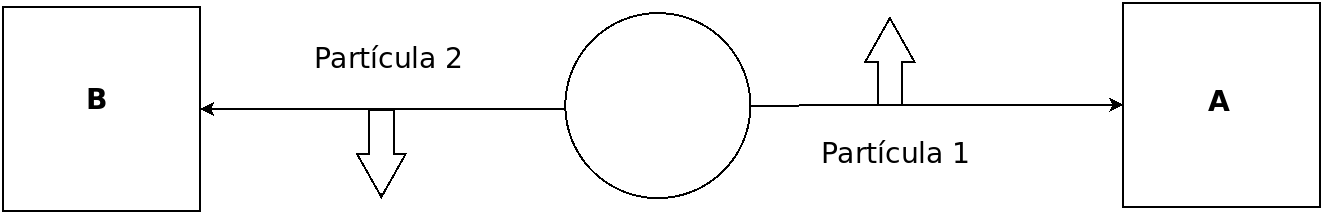
\includegraphics[scale=0.27]{./spin_correlation_spin_singlet.png} 
\end{center} 
\caption{Correlación de spin para un estado \textit{spin-singlet}}
\label{fig::spin_correlation_spin_singlet}
\end{figure}
Para un sistema de una partícula de spin $\frac{1}{2}$ se tienen los  eigenkets(vectores propios) $S_x$ y $S_z$ están relacionados de la siguiente manera \footnote{ver\ref{sec::appendix} o \cite{Sakurai}}
\begin{equation}
|\mathbf{\hat{x}\pm}\rangle=\frac{1}{\sqrt{2}}\big (|\mathbf{\hat{z}+}\rangle \pm |\mathbf{\hat{z}-}\rangle  \big),\,\,\,\,\,|\mathbf{\hat{z}\pm}\rangle=\frac{1}{\sqrt{2}}\big (|\mathbf{\hat{x}+}\rangle \pm |\mathbf{\hat{x}-}\rangle  \big).
\end{equation}
Continuando la discusión con el sistema compuesto, se puede reescribir el estado de spin-singlet \ref{eq::singlet_state} escogiendo al eje $x$ cómo eje de cuantización de la siguiente manera:
\begin{equation}
|\text{\textit{spin-singlet}}\rangle=\frac{1}{\sqrt{2}}\big( |\mathbf{\hat{x}}-;\mathbf{\hat{x}}+\rangle -|\mathbf{\hat{x}}+;\mathbf{\hat{x}}-\rangle  \big).
\end{equation}
está expresión es muy parecida a \ref{eq::singlet_state} y aparte del signo(que es una convención) se pudo esperaba tener una expresión análoga debido al hecho que para los estados de \textit{spin-singlet} no hay preferencia de dirección espacial. Suponiendo ahora que el observador A puede elegir medir $S_z$ or $S_x$ para la partícula 1 al cambiar la orientación de su dispositivo para medir el spin, mientras que el observador B se concentra en una sola dirección $S_x$ para la partícula 2. Si A mide $S_z$ y obtiene un valor positivo B tiene claramente $50\%-50\%$ chance de hallar $S_x\, +$ o $S_x\,-$ aunque se sepa que $S_z$ es con certeza negativo, su componente $S_x$ está totalmente indeterminado. Por el otro lado, suponiendo que A escoge medir $S_x$ entonces cuando mida un valor positivo para la partícula 1 el observador B tendrá con certeza un valor negativo para $S_x$. La última opción en la que el observador A prefiere no hacer ninguna medición sobre la partícula 1 entonces es claro que el observador B tiene de nuevo $50\%-50\%$ chance de medir $S_x\,+$ o $S_x\,-$, para resumirlo
\begin{enumerate}
\item Si A mide $S_z$ y B mide $S_x$, entonces hay una correlación completamente aleatoria entre las dos mediciones. 
\item Si A mide $S_x$ y B mide $S_x$, entonces hay una correlación perfecta(signos opuestos en las mediciones) entre las dos mediciones.
\item Si A no realiza medición, entonces las mediciones de B dan resultados aleatorios.
\end{enumerate}
Estos hechos demuestran que el resultado de la medición realizada por B parece depender de que tipo de medición el observador decide hacer: una medición de $S_x$, una medición de $S_y$, o ninguna medición. Es importante recalcar que A y B pueden estar ha kilómetros de distancia sin posibilidad de comunicación o alguna interacción. El observador A puede decidir la orientación de su dispositivo para medir el spin mucho después de que las partículas se separan. Pareciera ser que la partícula 2 ''sabe'' el componente del spin de la partícula 1 que se está midiendo instantáneamente. \\
La interpretación ortodoxa(la interpretación de Copenhagen) de está situación es la siguiente, la medición del observador A es un proceso de selección o filtrado. Cuando se mide $S_z$ de la partícula 1 y se obtiene un valor positivo, entonces se selecciona al componente $|\mathbf{\hat{z}}+;\mathbf{\hat{z}}-\rangle$ o la función de onda colapsa a este estado, una medición subsecuente de $S_z$ en la otra partícula tan sólo confirma que el estado es de hecho $|\mathbf{\hat{z}}+;\mathbf{\hat{z}}-\rangle$ o sigue en este estado. Se debe aceptar que lo que parece ser una medición en una parte del sistema es una medición en el sistema bipartito o el sistema completo.
\subsection{Principio de localidad de Einstein y la desigualdad de Bell}
Varios físicos han tenido una inconformidad o han tenido otras interpretaciones con respecto a la interpretación ortodoxa antes expuesta. Probablemente el más famoso siendo Albert Einstein que siempre mostró e hizo explícita su inconformidad con varios aspectos de la teoría cuántica. El principio de localidad de Einstein es el siguiente: La situación real es que el comportamiento del sistema $S_2$ es independiente del sistema $S_1$ que esta espacialmente separado del primer sistema y por lo tanto no tiene una influencia directa. Este problema fue discutido por primera vez en un artículo seminal que se conoce como la paradoja EPR(Einstein, Podolsky y Rosen) ver \cite{Einstein}. Algunos han argumentado que las dificultades o incongruencias encontradas en este fenómeno son inherentes de las interpretaciones probabilísticas de la mecánica cuántica y que el comportamiento de la dinámica a nivel microscópico aparenta ser probabilístico debido a que se desconocen algunos parámetros por descubrir que se han llamado \textbf{variables ocultas}(\textit{hidden variables}) no han sido especificados. Hay varias propuestas teóricas alternativas a la interpretación ortodoxa de la mecánica cuántica basadas en variables ocultas u otras consideraciones, por ejemplo la teoría de onda piloto de Bohm, introducida por uno de los padres de la teoría cuántica, Louis de Broglie. La pregunta fundamental para establecer la validez de la teoría cuántica es, ¿las teorías alternativas hacen predicciones que difieren de las hechas por la mecánica cuántica?. Hasta 1964 se creía que las teorías alternativas podían manipularse de tal forma que sus predicciones siempre coincidían  con las predicciones cuánticas, el debate se podía considerar en ese sentido un tópico metafísico o filosófico, al final los resultados experimentales eran idénticos. No fue hasta que John. S. Bell dedujo que las teorías alternativas basadas en el principio de localidad de Einstein producían predicciones en la forma de una relación de desigualdad entre los observables de experimentos de correlaciones de spin que estaba en desacuerdo con las predicciones para el mismo experimento derivadas de la interpretación ortodoxa de la mecánica cuántica que además podía ser sometida a confirmación experimental.\\
Aquí se derivan la relación de desigualdad de Bell en el marco de un modelo simple concebido inicialmente por Eugene Wigner, que incorpora todos los aspectos fundamentales de las teorías alternativas basadas en las variables ocultas. Los proponentes de este modelo aseguran que es imposible determinar $S_x$ y $S_y$ simultáneamente, i.e. son variables conjugadas. Sin embargo cuando se tiene un número grande de partículas con spin $\frac{1}{2}$ se asigna a cierta fracción de las partículas con la siguiente propiedad:
\begin{enumerate}
\item Si se mide $S_z$, se obtiene un valor positivo con certeza.
\item Si se mide $S_x$, se obtiene un valor negativo con certeza.
\end{enumerate}
Se dice que una partícula que satisface esta propiedad pertenece al tipo $(\mathbf{\hat{z}}+,\, \mathbf{\hat{x}}-)$, hay que notar con está propiedad no se está aseverando que se pueda medir simultáneamente a $S_x$ y $S_z$ y medir $+$ y $-$ respectivamente. Cuando se mide $S_x$ no mide $S_z$ y viceversa. Se asignan valores definidos para componentes del spin en más de una dirección con la aclaración que sólo se mide un componente a la vez. Aunque este acercamiento es fundamentalmente distinto al de la mecánica cuántica, las predicciones cuánticas para las mediciones de $S_x$ y $S_x$ para el spin arriba $(S_z+)$pueden ser reproducidas dado que se tienen tantas partículas que pertenecen al tipo $(\mathbf{\hat{z}}+,\, \mathbf{\hat{x}}+)$ cómo al tipo $(\mathbf{\hat{z}}+,\, \mathbf{\hat{x}}-)$.\\
Examinando cómo este modelo relativamente sencillo puede explicar las correlaciones en la mediciones hechas sobre sistemas compuestos por estados \textit{spin-singlets}, es claro que para un par en particular debe cumplirse o debe haber una correlación perfecta en la hay una coincidencia entre la partícula 1 y partícula 2 de tal manera que el momento angular del sistema es igual a cero: si la partícula 1 es del tipo $(\mathbf{\hat{z}}+,\, \mathbf{\hat{x}}-)$, entonces la partícula 2 es del tipo $(\mathbf{\hat{z}}-,\, \mathbf{\hat{x}}+)$, y de manera análoga en todos los otros casos(ver \cite{Sakurai}). Estos resultados de correlación pueden reproducirse si la partícula 1 y la partícula 2 coinciden de la siguiente manera:
\begin{equation}
\begin{aligned}
\text{partícula 1}\,\,\,\,\,\,\text{partícula 1}\\
(\mathbf{\hat{z}}+,\, \mathbf{\hat{x}}-) \leftrightarrow (\mathbf{\hat{z}}-,\, \mathbf{\hat{x}}+), 
\end{aligned}
\end{equation}
\begin{equation}\label{eq::type_1_singlet_state}
(\mathbf{\hat{z}}+,\, \mathbf{\hat{x}}+) \leftrightarrow (\mathbf{\hat{z}}-,\, \mathbf{\hat{x}}-),
\end{equation}
\begin{equation}
(\mathbf{\hat{z}}-,\, \mathbf{\hat{x}}+) \leftrightarrow (\mathbf{\hat{z}}+,\, \mathbf{\hat{x}}-),
\end{equation}
\begin{equation}
(\mathbf{\hat{z}}-,\, \mathbf{\hat{x}}-) \leftrightarrow (\mathbf{\hat{z}}+,\, \mathbf{\hat{x}}+),
\end{equation}
con proporciones iguales, $25\%$ cada una de las porciones de partículas. Se implica una suposición importante en este desarrollo, suponiendo que un par que pertenece al tipo \ref{eq::singlet_state} y el observador A decide hacer una medición del componente $S_z$ de la partícula 1, en este caso se obtiene un  valor positivo independientemente si el observador B decide medir $S_z$ o $S_x$. Es en este sentido en el que se incorpora el principio de localidad de Einstein en el modelo: el resultado de la medición de A está independientemente predeterminado de la elección que el observador B haga en su medición.\\
En los ejemplos considerados previamente, se han reproducido exitosamente las predicciones de la mecánica cuántica. Considerando situaciones más elaboradas en las que el modelo hace predicciones que difieren de las hechas por la teoría de la mecánica cuántica. En este caso más complejo se tienen tres vectores unitarios $\mathbf{\hat{a}}$, $\mathbf{\hat{b}}$ y $\mathbf{\hat{c}}$, que en general no son mutuamente ortogonales. Se tiene el caso en que una de las partículas pertenece al un grupo definido, por ejemplo $(\mathbf{\hat{a}}-,\, \mathbf{\hat{b}}+,\,\mathbf{\hat{c}}+)$, que significa que si se mide $\mathbf{S}\cdot \mathbf{\hat{a}}$, se obtiene un medición negativa con certeza; si se mide $\mathbf{S}\cdot \mathbf{\hat{b}}$ se obtiene una medición positiva con certeza y finalmente si se mide $\mathbf{S}\cdot \mathbf{\hat{c}}$ también se obtiene una medición positiva. De manera análoga que el caso en el que sólo se tiene dos direcciones en este caso debe de haber una coincidencia perfecta con la otra partícula, por conservación de momento angular del sistema, es decir que la partícula 2 es del tipo $(\mathbf{\hat{a}}+,\, \mathbf{\hat{b}}-,\,\mathbf{\hat{c}}-)$. En un caso aleatorio cualquiera el par de partículas debe de pertenecer a uno de los ocho tipos que se detallan en la tabla \ref{tab:three_direction_correlations}. Estas ocho posibilidades son mutuamente excluyentes y disjuntas\footnote{Conjuntos sin elementos en común.}. El número de partículas de cada tipo se especifica en la primera columna de la tabla. Para ilustrar cómo se calculan las probabilidades en este experimento se supone que el observador A hace una medición de $\mathbf{S_1}\cdot \mathbf{\hat{a}}$ y obtiene un valor positivo y el observador B hace una medición $\mathbb{S_2}\cdot \mathbf{\hat{b}}$ también positiva entonces es claro que de la tabla \ref{tab:three_direction_correlations} que el par de partículas sólo tiene puede pertenecer a dos grupos, el grupo 3 o el grupo 4 por lo que el número total de pares de partículas es $N_3 + N_4$. Debido a que $N_i\geq 0$, se tienen relaciones de desigualdad del tipo:
\begin{equation}\label{eq::positivity_condition}
N_3 + N_4 /geq (N_2 +  N_4) + (N_3 +  N_7)
\end{equation} 
Si $P(\mathbf{\hat{a}}+;\,\mathbf{\hat{b}}+)$ es la probabilidad que, en una selección aleatoria el observador A mida $\mathbf{S}\cdot \mathbf{\hat{a}}$ y obtenga $+$ y el observador B mida $\mathbf{S}\cdot \mathbf{\hat{b}}$ y obtenga $+$, y así de manera análoga para todas las otras combinaciones de posibilidades.	
\begin{table}
\centering
\begin{tabular}{|c|c|c|}
\hline
\toprule
\textbf{Grupo} & \textbf{Partícula 1} & \textbf{Partícula 1} \\
\midrule
$N_1$ & $(\mathbf{\hat{a}}+,\, \mathbf{\hat{b}}+,\,\mathbf{\hat{c}}+)$ & $(\mathbf{\hat{a}}-,\, \mathbf{\hat{b}}-,\,\mathbf{\hat{c}}-)$\\
$N_2$ & $(\mathbf{\hat{a}}+,\, \mathbf{\hat{b}}+,\,\mathbf{\hat{c}}-)$ & $(\mathbf{\hat{a}}-,\, \mathbf{\hat{b}}-,\,\mathbf{\hat{c}}+)$\\
$N_3$ & $(\mathbf{\hat{a}}+,\, \mathbf{\hat{b}}-,\,\mathbf{\hat{c}}+)$ & $(\mathbf{\hat{a}}-,\, \mathbf{\hat{b}}+,\,\mathbf{\hat{c}}-)$\\
$N_4$ & $(\mathbf{\hat{a}}+,\, \mathbf{\hat{b}}-,\,\mathbf{\hat{c}}-)$ & $(\mathbf{\hat{a}}-,\, \mathbf{\hat{b}}+,\,\mathbf{\hat{c}}+)$\\
$N_5$ & $(\mathbf{\hat{a}}-,\, \mathbf{\hat{b}}+,\,\mathbf{\hat{c}}+)$ & $(\mathbf{\hat{a}}+,\, \mathbf{\hat{b}}-,\,\mathbf{\hat{c}}-)$\\
$N_6$ & $(\mathbf{\hat{a}}-,\, \mathbf{\hat{b}}+,\,\mathbf{\hat{c}}-)$ & $(\mathbf{\hat{a}}+,\, \mathbf{\hat{b}}-,\,\mathbf{\hat{c}}+)$\\
$N_7$ & $(\mathbf{\hat{a}}-,\, \mathbf{\hat{b}}-,\,\mathbf{\hat{c}}+)$ & $(\mathbf{\hat{a}}+,\, \mathbf{\hat{b}}+,\,\mathbf{\hat{c}}-)$\\
$N_8$ & $(\mathbf{\hat{a}}-,\, \mathbf{\hat{b}}-,\,\mathbf{\hat{c}}-)$ & $(\mathbf{\hat{a}}+,\, \mathbf{\hat{b}}+,\,\mathbf{\hat{c}}+)$\\
\bottomrule
\hline
\end{tabular}
    \label{tab:three_direction_correlations}
\end{table}
La probabilidad está dada por 
\begin{equation}
P(\mathbf{\hat{a}}+;\, \mathbf{\hat{b}},+) = \frac{N_3+N_4}{\sum_{i=1}^{8} N_i} 
\end{equation}
De manera análoga se tiene que 
\begin{equation}
P(\mathbf{\hat{a}}+;\, \mathbf{\hat{c}},+) = \frac{N_2+N_4}{\sum_{i=1}^{8} N_i} 
\end{equation}
y
\begin{equation}
P(\mathbf{\hat{c}}+;\, \mathbf{\hat{b}},+) = \frac{N_3+N_7}{\sum_{i=1}^{8} N_i} 
\end{equation}
la condición de positividad del número de poblaciones en cada tipo \ref{eq::positivity_condition} da cómo resultado
\begin{equation}\label{eq::Bell_inequality}
P(\mathbf{\hat{a}}+;\, \mathbf{\hat{b}},+) \geq P(\mathbf{\hat{a}}+;\, \mathbf{\hat{c}},+) + P(\mathbf{\hat{c}}+;\, \mathbf{\hat{b}},+)  
\end{equation}
Está es la \textbf{desigualdad de Bell}, que es una consecuencia del principio de localidad de Einstein.

\subsection{Desigualdad de Bell y Mecánica Cuántica}
En el punto de vista de la Mecánica Cuántica no se habla de una fracción de pares de partículas por ejemplo $\frac{N_3}{\sum_{i=1}^{8} N_i}$ pertenecientes al tipo 3, en lugar de esto se caracteriza todos los sistemas de \textit{spin-singlet} por el mismo ket \ref{eq::singlet_state}, en este sentido se tiene un ensamble puro(ver Sakurai \cite{Sakurai}). Usando el ket \ref{eq::singlet_state} y las reglas de la mecánica cuántica se pueden calcular las probabilidades de la desigualdad de Bell \ref{eq::Bell_inequality} sin ninguna ambigüedad.\\

Primero se evalúa $P(\mathbf{\hat{a}}+;\, \mathbf{\hat{b}},+)$. Suponiendo que el observador A mide $\mathbf{\hat{S}} \cdot \mathbf{\hat{a}}$ y haya un valor $+$; debido a la correlación perfecta por la conservación del momento angular discutida previamente, la medición del observador B para $\mathbf{\hat{S}} \cdot \mathbf{\hat{b}}$ va a resultar en $-$ con certeza. Pero para calcular $P(\mathbf{\hat{a}}+;\, \mathbf{\hat{b}},+)$ se debe considerar un nuevo eje de cuantización para $\mathbf{\hat{b}}$ con un ángulo $\theta_{ab}$ con respecto a $\mathbf{\hat{a}}$, ver figura \ref{fig::P_evaluation}. 
\begin{figure}[h]
\begin{center}
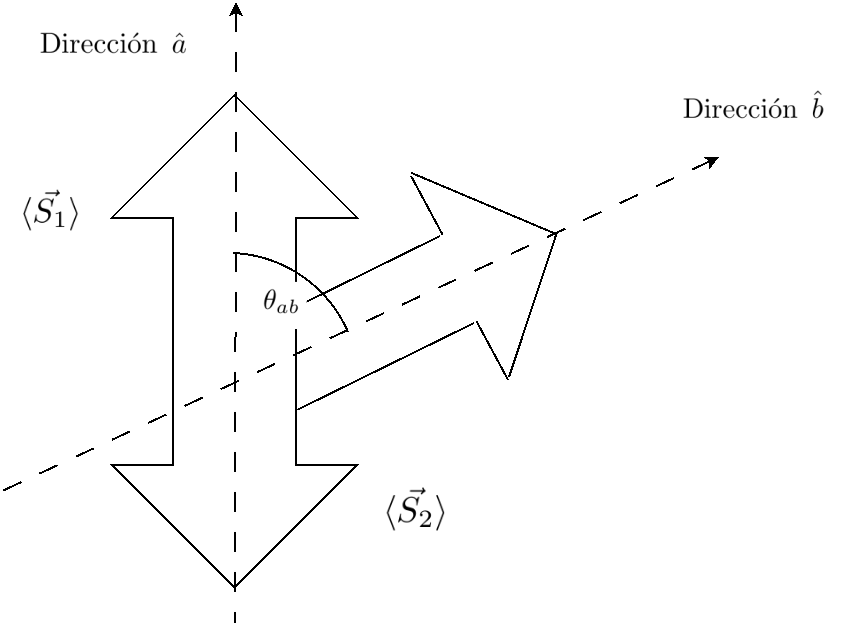
\includegraphics[scale=0.24]{./evaluation_P.png} 
\end{center} 
\caption{Evaluación de $P(\mathbf{\hat{a}}+;\, \mathbf{\hat{b}},+)$}
\label{fig::P_evaluation}
\end{figure}
De acuerdo al formalismo de la formulación matricial de la mecánica cuántica(ver \cite{Sakurai}), la probabilidad que la medición de $\mathbf{S}_2\cdot \mathbf{\hat{b}}$ de como resultado $+$ cuando se sabe que la partícula 2 es un estado propio(\textit{eigenvalue}) de $\mathbf{S}_2\cdot \mathbf{\hat{a}}$ con valor propio negativo está dado por
\begin{equation}
\cos^2\Bigg[\frac{\pi-\theta_{ab}}{2}\Bigg]=\sin^2\bigg(\frac{\theta_{ab}}{2}\bigg)
\end{equation}
Cómo resultado se obtiene que 
\begin{equation}\label{eq::P_ab_probability}
P(\mathbf{\hat{a}}+;\, \mathbf{\hat{b}},+)=\frac{1}{2}\sin^2\bigg(\frac{\theta_{ab}}{2}\bigg)
\end{equation}
donde el factor $\frac{1}{2}$ surge de la probabilidad inicial de obtener $\mathbf{S}_1\cdot \mathbf{\hat{a}}$ con valor $+$. Usando la expresión \ref{eq::P_ab_probability} y su generalización para los otros 2 términos de \ref{eq::Bell_inequality} se puede reescribir la desigualdad de Bell cómo:
\begin{equation}\label{eq::Bell_inequality_2}
\sin^2\bigg(\frac{\theta_{ab}}{2}\bigg)\leq \sin^2\bigg(\frac{\theta_{ac}}{2}\bigg)+\sin^2\bigg(\frac{\theta_{cb}}{2}\bigg)
\end{equation}

Con este resultado se puede demostrar que la desigualdad \ref{eq::Bell_inequality_2} no siempre se cumple desde un acercamiento geométrico. Por simplicidad se escoge a $\mathbf{\hat{a}}$, $\mathbf{\hat{b}}$ y $\mathbf{\hat{c}}$ a estar en un plano, y se escoge a $\mathbf{\hat{c}}$ de tal manera que bisecte las direcciones definidas por $\mathbf{\hat{a}}$ y $\mathbf{\hat{b}}$, con estas simplificaciones se obtiene:
\begin{equation}
\theta_{ab}=2\theta,\,\,\,\,\,\,\,\,\, \theta_{ac}=\theta_{cb}=\theta
\end{equation}
La desigualdad \ref{eq::Bell_inequality_2} es violada para
\begin{equation}
0<\theta<\frac{\pi}{2}
\end{equation}
Por ejemplo, si se toma $\theta=\frac{\pi}{4}$ se obtiene la contradicción
\begin{equation}
0.500\leq 0.292
\end{equation}
Con esto se puede evidenciar claramente que las predicciones de la mecánica cuántica no son compatibles con la desigualdad de Bell. Hay un observable real(en el sentido que puede verificarse experimentalmente) que difiere entre las predicciones cuánticas y la teoría alternativa que satisface el principio de localidad de Einstein.

%\section{Generalización del teorema de Bell}
\section{Desigualdad CHSH}
La desigualdad CHSH nombrada por las iniciales de los autores del teorema: Clauser, Horne, Shimony y Holt(ver \cite{Clauser}). Está desigualdad es usada experimentalmente para probar el teorema de Bell(\cite{Bell}). El teorema asegura que las teorías basadas en variables ocultas y el principio de localidad de Einstein no pueden explicar por completo las implicaciones y consecuencias del entrelazamiento en la mecánica cuántica.\\

El premio Nobel 2022 fue galardonado a Alain Aspect, John Clauser y Anton Zellinger por su trabajo de vanguardia en información cuántica y en particular por sus experimentos con fotones entrelazados cuánticamente que demostraron sin lugar a duda la violación de las desigualdades de Bell.\\

Para poder recrear este experimento en el contexto de la computación cuántica se crea un par de qubits entrelazados en dos bases distintas. Se etiqueta a la base del primer qubit $A$ y $a$ y a la segunda base $B$ y $b$. Esto permite computar la cantidad CHSH $S_1$ cómo:
\begin{equation}\label{eq::S_1}
S_1=A(B-b)+a(B+b)
\end{equation} 
cada observable puede tomar los valores $+1$ o $-1$ unicamente. Es claro que cada uno de los términos $B\pm b$ debe ser $0$ y el otro $\pm 2$. Por lo tanto $S_1=\pm 2$. El valor promedio de $S_1$ debe satisfacer la desigualdad
\begin{equation}\label{eq::CHSH_inequality_S1}
|\langle S_1 \rangle|\leq 2.
\end{equation}
Expandiendo en términos de $A, \, a,\, B$ y $b$ se obtiene
\begin{equation}\label{eq:CHSH_inequality_S1_2}
|\langle S_1 \rangle|=|\langle A B\rangle-\langle A b \rangle + \langle a B \rangle + \langle a b \rangle| \leq 2
\end{equation}
Se puede definir otra cantidad CHSH $S_2$ cómo:
\begin{equation}
S_2=A(B+b)-a(B-b)
\end{equation}
de nuevo expandiendo en términos de $A, \, a,\, B$ y $b$  lleva a otra desigualdad para el valor promedio de $S_2$
\begin{equation}\label{eq::CHSH_inequality_S2}
|\langle S_2 \rangle|=|\langle A B\rangle+\langle A b \rangle - \langle a B \rangle + \langle a b \rangle| \leq 2
\end{equation}
Si la mecánica cuántica puede describirse por teorías de variables ocultas y el principio de localidad de Einstein, la desigualdades \ref{eq:CHSH_inequality_S1_2} y \ref{eq::CHSH_inequality_S2} deben de cumplirse. Sin embargo se pueden usar ordenadores cuánticos para demostrar que estás desigualdades son violadas por lo que se puede concluir de los experimentos que aquí se detallan que la teoría cuántica no es compatible con teorías de variables ocultas locales.
\subsection{Violación de las desigualdades CHSH}
Para demostrar la violación de las desigualdades CHSH se imagina a Alice y Bob se les da a cada uno, una parte de un sistema bipartito entrelazado cuánticamente. Cada uno de ellos realiza dos mediciones en su parte del sistema en dos bases distintas. Para continuar con el desarrollo presentado anteriormente se llama a la bases de Alice $A$ y $a$ y las bases en las que mide Bob $B$ y $b$. Entonces Alice y Bob tienen un qubit cada uno, por lo que cualquier medición puede resultar unicamente en $\pm 1$, típicamente se refiere a estos qubits cómo $|0\rangle$ y $|0\rangle$ se hace el recordatorio que estos son estados propios(\textit{eigenstates}) y una medición proyectiva resulta en los valores propios $+1$ y $-1$, respectivamente.\\

La discusión anterior está un tanto sobresimplificada, ya que puede considerase que el resultado de un conjunto de mediciones de Alice y Bob pueden depender de un conjunto de variables ocultas locales, pero se puede demostrar con algunos desarrollos matemáticos(ver \cite{Clauser}), que incluso cuando ese es el caso el valor esperado o promedio de \ref{eq::CHSH_inequality_S1_2} y \ref{eq::CHSH_inequality_S2} no puede exceder el valor impuesto por las desigualdades referidas es decir que está limitado a dar cómo máximo el valor de $2$ si el principio de localidad de Einstein es valido también conocido como realismo local.\\

El primer paso para probar estas desigualdades es construir el observable \ref{eq::S_1} donde $A$, $a$ son cada uno de los operadores $\{IX, IZ\}$\footnote{$I$ es la identidad y $X$ y $Z$ son los operadores de Pauli $S_x$ y $S_z$ respectivamente} para el qubit de Alice o el qubit $0$; y para $B$, $b$ se tiene que son $\{XI, ZI\}$ para el qubit de Bob o el qubit $1$.
\subsection{Implementación en Qiskit}
En la plataforma de computación cuántica Qiskit los operadores de Pauli en distintos qubits pueden construirse al especificar el orden de los operadores con una secuencia de caracteres, por ejemplo al instanciar al objeto de las librerías de Qiskit llamado \texttt{SparsePauliOp} con la secuencia de caracteres \texttt{'ZX'} cómo argumento se implica una medición de $\langle X \rangle$ en el qubit \texttt{q0} y una medición $\langle Z \rangle$ en el qubit \texttt{q1}. Este producto tensorial, que se puede entender cómo combinar operadores para distintos qubits del sistema bipartito puede implementarse explícitamente usando el método de Qiskit \texttt{.tensor()}, adicionalmente se pueden combinar operadores que actúan sobre el mismo qubit con el método \texttt{.compose()}. Por ejemplo todos los siguientes comandos crean el mismo operador de Pauli

\VerbatimInput{pauli_example.txt}


Con está breve introducción a la versatilidad de Qiskit el primer paso para hacer el experimento en un ordenador cuántico es crear el operador para un testigo CHSH utilizando \texttt{SparsePauliOp}, el código es relativamente sencillo

\VerbatimInput{observable}

Después se construye un par de qubits entrelazados al crear el estado de Bell(ver \cite{Medina})
\begin{equation}\label{eq::Bell_state}
|\Phi^{+}\rangle=\frac{|00\rangle+|11\rangle}{\sqrt{2}}
\end{equation}
Usando la primitiva \texttt{Estimator} de Qiskit se pueden obtener relativamente fácil los valores esperados necesarios: $(\langle AB \rangle, \langle Ab\rangle, \langle aB \rangle, \langle ab\rangle)$. Habiendo calculado estos valores esperado se pueden calcular las dos cantidades CHSH $\langle S_1\rangle$ y $\langle S_2\rangle$.\\

Para crear el estado de Bell \ref{eq::Bell_state} se necesita utilizar un compuerta de Hadamard seguido por una compuerta \texttt{CNOT}(ver \cite{Medina}) con qubit el mismo qubit objetivo al cual se ha operado con el operador de Hadamard. Debido a la simplificación discutida previamente en la que solo se hacen mediciones en las bases $X$ y $Z$ se necesita hacer una rotación del estado de Bell alrededor de la esfera de Bloch que equivale a cambiar la base de medición(ver \cite{Qiskit}). Esto puede lograrse aplicando una compuerta $R_y(\theta)$, donde $\theta$ es un parámetro(\texttt{Parameter}) a ser especificado por el una llamada a la API del \texttt{Estimator}. Esto resulta en el estado
\begin{equation}\label{eq::psi_state}
|\psi\rangle=\frac{1}{\sqrt{2}}\Bigg((\cos\bigg(\frac{\theta}{2} \bigg))|00\rangle+\sin\bigg(\frac{\theta}{2} \bigg))|11\rangle\Bigg)
\end{equation}
El código de Python que implementa el estado \ref{eq::psi_state} es el siguiente:
\VerbatimInput{psi_state.txt}
El circuito cuántico correspondiente se visualiza en la siguiente figura
\begin{figure}[h]
\begin{center}
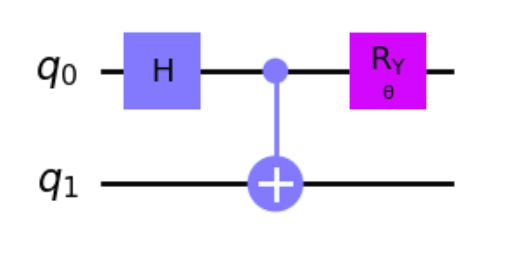
\includegraphics[scale=0.2]{./psi_state_circuit.png} 
\end{center} 
\caption{Circuito cuántico para construir \ref{eq::psi_state}}
\label{fig::psi_state_circuit}
\end{figure}
\pagebreak
%\section{Apéndice}\label{sec::appendix}


\begin{thebibliography}{99}
%% La bibliografía se ordena en orden alfabético respecto al apellido del 
%% autor o autor principal
%% cada entrada tiene su formatado dependiendo si es libro, artículo,
%% tesis, contenido en la web, etc
\bibitem{Arfken} George Arfken. \textit{Mathematical Methods for Physicists}.

\bibitem{Bell} J.S. Bell. \textit{On the Einstein Podolski Rosen Paradox}. \url{https://cds.cern.ch/record/111654/files/vol1p195-200_001.pdf}

\bibitem{Clauser} John F. Clauser, Michael A. Horne, Abner Shimony, Richard Holt. \textit{PROPOSED EXPERIMENT TO TEST LOCAL HIDDEN-VARIABLE THEORIES.}. Physical Review Letters,. 23(15):880-4, \url{https://journals.aps.org/prl/abstract/10.1103/PhysRevLett.23.880}.

\bibitem{Einstein} Einstein A., B. Podolsky, N. Rosen, \textit{Can Quantum-Mechanical Description of Physical Reality be Considered Complete?}. Physical Review. \url{doi:10.1103/PhysRev.47.777}

\bibitem{Medina} Julio Medina. \textit{Reporte de Seminario 1. Computación Cuántica}. \url{https://github.com/Julio-Medina/Seminario/blob/main/Reporte_final/reporte_final.pdf}

\bibitem{Nielsen} Michael A. Nielsen, Isaac L. Chuang. \textit{Quantum Computation adn Quantum Information}. Cambridge University Press 2010. 10th. Anniversary Edition.

\bibitem{Feynman} Richard P. Feynman. \textit{Simulating Physics with Computers.} \url{https://doi.org/10.1007/BF02650179}.

\bibitem{Qiskit} \textit{Qiskit Textbook}. \url{https://qiskit.org/textbook-beta}

\bibitem{Mermin} N. David Mermin \textit{Quantum Computer Science: An Introduction}. Cambridge University Press, 2007.

\bibitem{Sakurai} J.J. Sakurai \textit{Modern Quantum Mechanics}. The Benjamin/Cummings Publishing Company, 1985.

\bibitem{Dotsenko} Viktor Dotsenko. \textit{An Introduction to the Theory of Spin Glasses and Neural Networks}. World Scientific 1994.

\bibitem{Bahri} Yasaman Bahri, Jonathan Kadmon, Jeffrey Pennington, Sam S. Schoenholz, Jascha Sohl-Dickstein, Surya Ganguli. \textit{Statistical Mechanics of Deep Learning}. \url{https://www.annualreviews.org/doi/pdf/10.1146/annurev-conmatphys-031119-050745}

\bibitem{openQASM} OpenQASM. \url{https://github.com/openqasm/openqasm}.
 

\end{thebibliography}
\end{document}

